% Options for packages loaded elsewhere
\PassOptionsToPackage{unicode}{hyperref}
\PassOptionsToPackage{hyphens}{url}
%
\documentclass[
  man]{apa6}
\usepackage{amsmath,amssymb}
\usepackage{lmodern}
\usepackage{iftex}
\ifPDFTeX
  \usepackage[T1]{fontenc}
  \usepackage[utf8]{inputenc}
  \usepackage{textcomp} % provide euro and other symbols
\else % if luatex or xetex
  \usepackage{unicode-math}
  \defaultfontfeatures{Scale=MatchLowercase}
  \defaultfontfeatures[\rmfamily]{Ligatures=TeX,Scale=1}
\fi
% Use upquote if available, for straight quotes in verbatim environments
\IfFileExists{upquote.sty}{\usepackage{upquote}}{}
\IfFileExists{microtype.sty}{% use microtype if available
  \usepackage[]{microtype}
  \UseMicrotypeSet[protrusion]{basicmath} % disable protrusion for tt fonts
}{}
\makeatletter
\@ifundefined{KOMAClassName}{% if non-KOMA class
  \IfFileExists{parskip.sty}{%
    \usepackage{parskip}
  }{% else
    \setlength{\parindent}{0pt}
    \setlength{\parskip}{6pt plus 2pt minus 1pt}}
}{% if KOMA class
  \KOMAoptions{parskip=half}}
\makeatother
\usepackage{xcolor}
\IfFileExists{xurl.sty}{\usepackage{xurl}}{} % add URL line breaks if available
\IfFileExists{bookmark.sty}{\usepackage{bookmark}}{\usepackage{hyperref}}
\hypersetup{
  pdftitle={The Presence of Objectification in Heterosexual Relationships},
  pdfauthor={Vivian Almaraz1, AJ Haller1, \& Alejandra Munoz1},
  pdflang={en-EN},
  hidelinks,
  pdfcreator={LaTeX via pandoc}}
\urlstyle{same} % disable monospaced font for URLs
\usepackage{longtable,booktabs,array}
\usepackage{calc} % for calculating minipage widths
% Correct order of tables after \paragraph or \subparagraph
\usepackage{etoolbox}
\makeatletter
\patchcmd\longtable{\par}{\if@noskipsec\mbox{}\fi\par}{}{}
\makeatother
% Allow footnotes in longtable head/foot
\IfFileExists{footnotehyper.sty}{\usepackage{footnotehyper}}{\usepackage{footnote}}
\makesavenoteenv{longtable}
\usepackage{graphicx}
\makeatletter
\def\maxwidth{\ifdim\Gin@nat@width>\linewidth\linewidth\else\Gin@nat@width\fi}
\def\maxheight{\ifdim\Gin@nat@height>\textheight\textheight\else\Gin@nat@height\fi}
\makeatother
% Scale images if necessary, so that they will not overflow the page
% margins by default, and it is still possible to overwrite the defaults
% using explicit options in \includegraphics[width, height, ...]{}
\setkeys{Gin}{width=\maxwidth,height=\maxheight,keepaspectratio}
% Set default figure placement to htbp
\makeatletter
\def\fps@figure{htbp}
\makeatother
\setlength{\emergencystretch}{3em} % prevent overfull lines
\providecommand{\tightlist}{%
  \setlength{\itemsep}{0pt}\setlength{\parskip}{0pt}}
\setcounter{secnumdepth}{-\maxdimen} % remove section numbering
% Make \paragraph and \subparagraph free-standing
\ifx\paragraph\undefined\else
  \let\oldparagraph\paragraph
  \renewcommand{\paragraph}[1]{\oldparagraph{#1}\mbox{}}
\fi
\ifx\subparagraph\undefined\else
  \let\oldsubparagraph\subparagraph
  \renewcommand{\subparagraph}[1]{\oldsubparagraph{#1}\mbox{}}
\fi
\newlength{\cslhangindent}
\setlength{\cslhangindent}{1.5em}
\newlength{\csllabelwidth}
\setlength{\csllabelwidth}{3em}
\newlength{\cslentryspacingunit} % times entry-spacing
\setlength{\cslentryspacingunit}{\parskip}
\newenvironment{CSLReferences}[2] % #1 hanging-ident, #2 entry spacing
 {% don't indent paragraphs
  \setlength{\parindent}{0pt}
  % turn on hanging indent if param 1 is 1
  \ifodd #1
  \let\oldpar\par
  \def\par{\hangindent=\cslhangindent\oldpar}
  \fi
  % set entry spacing
  \setlength{\parskip}{#2\cslentryspacingunit}
 }%
 {}
\usepackage{calc}
\newcommand{\CSLBlock}[1]{#1\hfill\break}
\newcommand{\CSLLeftMargin}[1]{\parbox[t]{\csllabelwidth}{#1}}
\newcommand{\CSLRightInline}[1]{\parbox[t]{\linewidth - \csllabelwidth}{#1}\break}
\newcommand{\CSLIndent}[1]{\hspace{\cslhangindent}#1}
\ifLuaTeX
\usepackage[bidi=basic]{babel}
\else
\usepackage[bidi=default]{babel}
\fi
\babelprovide[main,import]{english}
% get rid of language-specific shorthands (see #6817):
\let\LanguageShortHands\languageshorthands
\def\languageshorthands#1{}
% Manuscript styling
\usepackage{upgreek}
\captionsetup{font=singlespacing,justification=justified}

% Table formatting
\usepackage{longtable}
\usepackage{lscape}
% \usepackage[counterclockwise]{rotating}   % Landscape page setup for large tables
\usepackage{multirow}		% Table styling
\usepackage{tabularx}		% Control Column width
\usepackage[flushleft]{threeparttable}	% Allows for three part tables with a specified notes section
\usepackage{threeparttablex}            % Lets threeparttable work with longtable

% Create new environments so endfloat can handle them
% \newenvironment{ltable}
%   {\begin{landscape}\centering\begin{threeparttable}}
%   {\end{threeparttable}\end{landscape}}
\newenvironment{lltable}{\begin{landscape}\centering\begin{ThreePartTable}}{\end{ThreePartTable}\end{landscape}}

% Enables adjusting longtable caption width to table width
% Solution found at http://golatex.de/longtable-mit-caption-so-breit-wie-die-tabelle-t15767.html
\makeatletter
\newcommand\LastLTentrywidth{1em}
\newlength\longtablewidth
\setlength{\longtablewidth}{1in}
\newcommand{\getlongtablewidth}{\begingroup \ifcsname LT@\roman{LT@tables}\endcsname \global\longtablewidth=0pt \renewcommand{\LT@entry}[2]{\global\advance\longtablewidth by ##2\relax\gdef\LastLTentrywidth{##2}}\@nameuse{LT@\roman{LT@tables}} \fi \endgroup}

% \setlength{\parindent}{0.5in}
% \setlength{\parskip}{0pt plus 0pt minus 0pt}

% \usepackage{etoolbox}
\makeatletter
\patchcmd{\HyOrg@maketitle}
  {\section{\normalfont\normalsize\abstractname}}
  {\section*{\normalfont\normalsize\abstractname}}
  {}{\typeout{Failed to patch abstract.}}
\patchcmd{\HyOrg@maketitle}
  {\section{\protect\normalfont{\@title}}}
  {\section*{\protect\normalfont{\@title}}}
  {}{\typeout{Failed to patch title.}}
\makeatother
\shorttitle{Objectification in Heterosexual Relationships}
\DeclareDelayedFloatFlavor{ThreePartTable}{table}
\DeclareDelayedFloatFlavor{lltable}{table}
\DeclareDelayedFloatFlavor*{longtable}{table}
\makeatletter
\renewcommand{\efloat@iwrite}[1]{\immediate\expandafter\protected@write\csname efloat@post#1\endcsname{}}
\makeatother
\usepackage{csquotes}
\ifLuaTeX
  \usepackage{selnolig}  % disable illegal ligatures
\fi

\title{The Presence of Objectification in Heterosexual Relationships}
\author{Vivian Almaraz\textsuperscript{1}, AJ Haller\textsuperscript{1}, \& Alejandra Munoz\textsuperscript{1}}
\date{}


\affiliation{\vspace{0.5cm}\textsuperscript{1} Smith College}

\abstract{
The current study used dyadic analyses that considered each individual's objectification of themselves, the degree to which each individual objectifies their partner, and each partner's relationship satisfaction. Not many studies include perspective from both partners in a relationship, and not many studies consider both an individual's objectification of themselves and the objectification of the partner. To the best of our knowledge this is the first study to take a dyadic approach to investigating how both self and other objectification explain relationship satisfaction within heterosexual relationships. We found no evidence to support that an individual's objectification of their partner negatively influences relationship satisfaction for both men and women. Additionally, we also found no evidence to support our hypothesis that there is a stronger association between partner objectification and relationship satisfaction for women's relationship satisfaction than for men's. However, our results did find that a man's objectification of himself has a negative effect on his relationship satisfaction, meaning that the more the man objectifies himself, the less happy he will be in his relationship. The same was not found for women, as there was no significant relationship found between a woman's self-objectification and her own relationship satisfaction at all.We hope that in an effort to promote quality relationships, our research inspires greater consideration of self objectification in men, and in women.
}



\begin{document}
\maketitle

According to objectification theory, women are more socialized than men to internalize the observer's perspective of their bodies and their physical appearance (Fredrickson \& Roberts, 1997). The objectification of women can negatively impact women's mental health (Fredrickson \& Roberts, 1997). This internalization of the observer's perspective may be related to a woman hyper-focusing on her own appearance, and the objectification of herself. Self objectification is an individual's perception of themselves in which they prioritize physical appearance over physical ability (Sciangula \& Morry, 2009). Research shows that objectifying oneself and one objectifying their partner are highly associated with one another (Zurbriggen, Ramsey, \& Jaworski, 2011). This has been found to create sexual pressure for women in relationships (Ramsey \& Hoyt, 2015). Yet many studies have shown that objectification within heterosexual relationships often negatively affects both partners' relationship satisfaction (Mahar, Webster, \& Markey, 2020; Ramsey \& Hoyt, 2015; Ramsey, Marotta, \& Hoyt, 2017; Sáez, Riemer, Brock, \& Gervais, 2019). The current study explored the differences in objectification between partners in heterosexual relationships and how this influences each partner's relationship satisfaction. We believe that the association between relationship satisfaction and the objectification of an individual's partner is dependent on self objectification. Objectification research mostly considers the objectification of women outside of the context of relationships, so we have attempted to understand how objectification of oneself and one's partner influences relationship satisfaction in hopes of improving relationship quality.

The current study used dyadic analyses that considered each individual's objectification of themselves, the degree to which each individual objectifies their partner, and each partner's relationship satisfaction. Not many studies include perspective from both partners in a relationship, and not many studies consider both an individual's objectification of themselves and the objectification of the partner. To the best of our knowledge this is the first study to take a dyadic approach to investigating how both self and other objectification explain relationship satisfaction within heterosexual relationships. We hope that our research can provide insight as to how men and women objectify themselves and their partner, and how this explains satisfaction in their relationship.

Research on the effects of objectification of women in relationships have concluded different ideas. There is research that supports objectification theory, in which the objectification of women has negative implications, and there is research that suggests otherwise. Women who are sexually objectified by their partner are more likely to perceive their partner as less likable, are less likely to affiliate with their partner (Teng, Chen, Poon, \& Zhang, 2015), are more likely to experience body shame (Ramsey \& Hoyt, 2015) and have decreased relationship, body, and sexual satisfaction (Sáez et al., 2019). Alternative literature suggests that women can be satisfied in their relationships even while being objectified by their partners, and objectification is not inherently harmful towards relationship quality. Meltzer, McNulty, and Maner (2017) have found that in heterosexual relationships, women's marriage satisfaction and their husband's sexual valuation is moderated by the husband's relationship commitment. When a husband's marriage commitment is high, a women is more satisfied in her marriage and the husband sexually values her more (Meltzer \& McNulty, 2014; Meltzer et al., 2017). In another scenario observed in heterosexual relationships, women feel less objectified and enjoy the objectication by their partner compared to a stranger, colleague, or friend when women receive objectifying comments from them (Lameiras-Fernández, Fiske, Fernández, \& Lopez, 2018). Lameiras-Fernández suggests that women's perception of being objectified depends on the level of psychological intimacy with the objectifier. These results are surprising because the majority of research on objectification theory highlights the negative implications of objectification within relationships, so why does alternative research suggest otherwise? It is important to establish that partner objectification in relationships does not always have negative implications, and other factors such as psychological intimacy or self objectification can influence how objectification from a partner is perceived. The current study has pushed beyond previous research. Not only has this study explored partner objectification with dyadic analyses, but has also included perceived self regard, or self objectification to mediate this relationship.

Self objectification consistently serves as an important factor of relationship satisfaction in heterosexual relationships. Levels of self esteem influences individuals perceptions of themselves and their self objectification, and this perceived self regard predicts less relationship satisfaction (Sciangula \& Morry, 2009). Research has found that the more individuals within a partnership self-objectify, the lower they judge the quality of the relationship (Strelan \& Pagoudis, 2018), and are more likely to objectify their partners (Strelan \& Hargreaves, 2005). Additionally, Zurbriggen et al. (2011) has also found that an individual objectified by their partners are more likely to objectify themselves. This research suggests that there is a relationship between self objectification and partner objectification. Not only does self objectification interact with relationship satisfaction, but partner objectification is related to relationship satisfaction, as cited earlier. To the best of our knowledge, not many studies have considered both self objectification and partner objectification in relationship satisfaction research, nor have other studies considered how relationship satisfaction and partner objectification may depend on self objectification. Unlike previous studies, the current study went beyond past studies and included self objectification as a mediating role in the model.

A large majority of prior studies on self objectification focus exclusively on these effects on women. For example, women still tend to feel guilty or experience body shame if they enjoy being sexualized (Visser, Sultani, Choma, \& Pozzebon, 2014), they are more likely to feel objectified if they enjoy sexualization (Ramsey et al., 2017), and they experience more body surveillance, body shame, and body dissatisfaction than men (Choma et al., 2010; Gervais, Vescio, \& Allen, 2011). Women are also more cognizant of self-objectification than men (Newheiser, LaFrance, \& Dovidio, 2010) and are more affected in their current relationship by previous encounters of objectification (Terán, Jiao, \& Aubrey, 2021) than men. However, research shows that for men, an increase in body surveillance and body shame is associated with less social and romantic relationship pathways (Cole, Davidson, \& Gervais, 2013). Although much of the prior research focuses heavily on women and self objectification, self objectification is still present in men. Objectification theory emphasizes the consequential societal pressures only on women, but it is important to also consider men's perspective of objectifation because the research is in the context of heterosexual relationships . Accordingly, this current study included gender as a moderator in the relationships between partner objectification, self objectification, and relationship satisfaction.

\hypertarget{the-current-research}{%
\subsection{The Current Research}\label{the-current-research}}

Previous research has explored how the objectification of one's partner negatively influences relationship satisfaction, and how perceived self regard, self objectification, is also negatively related to relationship satisfaction for both men and women in hereosexual relationships(Sáez et al., 2019; Sciangula \& Morry, 2009). Consistent with previous research, we expect an individual's objectification of their partner will negatively influence relationship satisfaction for both men and women. It has been found that both men and women who self-objectify have higher tendencies to objectifying others (Strelan \& Hargreaves, 2005). Higher self and other objectification have a strong correlation with lower body satisfaction in women, but the same cannot be said for men (Strelan \& Hargreaves, 2005). Men and women interact with self and partner objectification differently, and much of the current literature focuses on the way women interact with objectification. In order to understand how relationship quality can be improved, it is important to consider how men experience objectification and objectify others. We wish to explore these differences in gender in our study. We hypothesize there will be a stronger association between partner objectification and relationship satisfaction for women's relationship satisfaction than for men.

Previous studies have not considered self objectification as a mediator between partner objectification and relationship satisfaction. Research shows that self objectification and partner objectification are positively associated with one another (Zurbriggen et al., 2011). Separate studies have found that objectifyng ones partner and self objectifying both decrease one's relationship satisfaction in a heterosexual relationship (Sáez et al., 2019; Sciangula \& Morry, 2009). Given the findings of previous studies, self objectification, partner objectification, and relationship satisfaction have associations with one another, and we suspect that partner objectification and relationship satisfaction would be dependent on one's perceived regard for themselves. We hypothesize that the association between men's objectification of his partner and his partner's relationship satisfaction will be mediated by women's objectification of herself. On the other hand, we expect that the association between women's objectification of her partner and her partner's relationship satisfaction will be mediated by men's objectification of himself. To our knowledge, this is the first study to mediate self objectification and moderate gender as part of a dyadic analysis. This current study investigated objectification of both individual and partner influence relationship satisfaction within heterosexual relationships across gender. We hope to understand how partners can be satisfied in their relationships, improve relationship quality, and highlight how objectification differs between gender.

\hypertarget{hypotheses}{%
\subsection{Hypotheses}\label{hypotheses}}

\begin{enumerate}
\def\labelenumi{\arabic{enumi}.}
\item
  An individual's objectification of their partner will negatively influence relationship satisfaction for both men and women.
\item
  There will be a stronger association between partner objectification and relationship satisfaction for women's relationship satisfaction than for men.
\item
  The association between men's objectification of his partner and his partner's relationship satisfaction will be mediated by women's objectification of herself.
\item
  The association between women's objectification of her partner and her partner's relationship satisfaction will be mediated by men's objectification of himself.
\end{enumerate}

\hypertarget{methods}{%
\section{Methods}\label{methods}}

\hypertarget{participants}{%
\subsection{Participants}\label{participants}}

\begin{longtable}[]{@{}
  >{\raggedright\arraybackslash}p{(\columnwidth - 6\tabcolsep) * \real{0.3952}}
  >{\centering\arraybackslash}p{(\columnwidth - 6\tabcolsep) * \real{0.2016}}
  >{\centering\arraybackslash}p{(\columnwidth - 6\tabcolsep) * \real{0.2016}}
  >{\centering\arraybackslash}p{(\columnwidth - 6\tabcolsep) * \real{0.2016}}@{}}
\caption{Demographic Data}\tabularnewline
\toprule
\begin{minipage}[b]{\linewidth}\raggedright
\end{minipage} & \begin{minipage}[b]{\linewidth}\centering
Man (N=173)
\end{minipage} & \begin{minipage}[b]{\linewidth}\centering
Woman (N=173)
\end{minipage} & \begin{minipage}[b]{\linewidth}\centering
Total (N=346)
\end{minipage} \\
\midrule
\endfirsthead
\toprule
\begin{minipage}[b]{\linewidth}\raggedright
\end{minipage} & \begin{minipage}[b]{\linewidth}\centering
Man (N=173)
\end{minipage} & \begin{minipage}[b]{\linewidth}\centering
Woman (N=173)
\end{minipage} & \begin{minipage}[b]{\linewidth}\centering
Total (N=346)
\end{minipage} \\
\midrule
\endhead
\textbf{Race} & & & \\
Asian or Asian American & 15 (8.7\%) & 20 (11.6\%) & 35 (10.1\%) \\
Black or African American & 11 (6.4\%) & 11 (6.4\%) & 22 (6.4\%) \\
Latinx or Hispanic & 10 (5.8\%) & 9 (5.2\%) & 19 (5.5\%) \\
Middle Eastern & 0 (0.0\%) & 2 (1.2\%) & 2 (0.6\%) \\
Other & 0 (0.0\%) & 1 (0.6\%) & 1 (0.3\%) \\
Prefer not to answer & 3 (1.7\%) & 1 (0.6\%) & 4 (1.2\%) \\
White or European American & 132 (76.3\%) & 127 (73.4\%) & 259 (74.9\%) \\
White or European American, Latinx or Hispanic & 2 (1.2\%) & 2 (1.2\%) & 4 (1.2\%) \\
\textbf{Age} & & & \\
Mean (SD) & 46.890 (8.790) & 44.803 (7.743) & 45.847 (8.337) \\
Range & 26.000 - 74.000 & 30.000 - 65.000 & 26.000 - 74.000 \\
\textbf{Sexual Orientation} & & & \\
Bisexual & 2 (1.2\%) & 6 (3.5\%) & 8 (2.3\%) \\
Heterosexual & 171 (98.8\%) & 167 (96.5\%) & 338 (97.7\%) \\
\textbf{Marriage} & & & \\
Let me explain\ldots{} & 0 (0.0\%) & 1 (0.6\%) & 1 (0.3\%) \\
No & 14 (8.1\%) & 15 (8.7\%) & 29 (8.4\%) \\
Yes & 159 (91.9\%) & 157 (90.8\%) & 316 (91.3\%) \\
\textbf{Income} & & & \\
N-Missing & 24 & 37 & 61 \\
Mean (SD) & 75610.128 (56807.296) & 64715.125 (75348.492) & 70411.109 (66409.273) \\
Range & 0.000 - 540000.000 & 0.000 - 750000.000 & 0.000 - 750000.000 \\
\bottomrule
\end{longtable}

Our sample started off with 182 couples (N=364). We decided to focus our study on heterosexual couples, leading us to exclude 9 same-sex couples from the sample, leaving us with 173 heterosexual couples (N=346). In our study, we asked the couples to answer questions about the role objectification had in their relationship and about their satisfaction within their relationship. All participants were over the age of 18 and in cohabitation with their partners. The majority (75\%) of the participants identified as White, 10\% were Asian, 6\% were Black, and 5\% were Hispanic. Other races accounted for the remaining 3\%. The participants' ages varied from 26 years of age to 74, with the participants being on average 45.8 years old (sd=8 years), and their income ranged from 0 dollars to 750,000 dollars. \emph{Refer to table 1 for more information.}

\hypertarget{measures}{%
\subsection{Measures}\label{measures}}

\begin{table}[tbp]

\begin{center}
\begin{threeparttable}

\caption{\label{tab:unnamed-chunk-2}}

\footnotesize{

\begin{tabular}{llllll}
\toprule
 & \multicolumn{1}{c}{M} & \multicolumn{1}{c}{SD} & \multicolumn{1}{c}{Relationship Quality} & \multicolumn{1}{c}{Self Objectification} & \multicolumn{1}{c}{Other Objectification}\\
\midrule
Relationship Quality & 7.43 & 1.50 & 1 &  & \\
Self Objectification & -1.27 & 2.24 & -0.07 & 1 & \\
Other Objectification & -0.73 & 2.23 & 0.06 & 0.31 & 1\\
\bottomrule
\end{tabular}

}

\end{threeparttable}
\end{center}

\end{table}

\textbf{Relationship satisfaction.} Relationship satisfaction is measured with the Relationship Questionnaire (Braiker \& Kelley, 1979). Ten out of the 30 items in the relationship questionnaire were used to measure feelings of love within the relationship. The love scale in the relationship questionnaire reflects the degree to which partners within a relationship express concern, feel a sense of belonging, attachment, and closeness. Example items of this scale include ``To what extent did you love your partner at this stage?'', ``How committed do you feel towards your partner?'' and ``How much do you feel you gave to the relationship?.'' Items were measured on a scale from 1- not at all to 9- very much. This scale was reliable, with a Cronbach's alpha of 0.93. The intraclass correlation coefficient for relationship satisfaction was significant, ICC = 0.698. \emph{Refer to Table 2 for more information.}

\textbf{Objectification.} Both self and other objectification was measured with the Self-Objectification Questionnaire (Noll \& Fredrickson, 1998). Each participant completed the questionnaire two times, first based on how they feel about themselves, and then how feel about their partner. The Self-Objectification Questionnaire asks participants to rank the extent to which they perceive their bodies and partner's bodies by appearance, and by physical ability. Some of these items include weight, physical attractiveness, overall health, and strength. Participants rank these ten aspects from 10 being most important, to 1 being least important. The intraclass correlation coefficient for self objectification was low, ICC = 0.241, and the intraclass correlation coefficient for other objectification was also low, ICC = 0.181. The self and other objectification scales are personality measures so we do not expect the intraclass coefficients to be highly correlated. \emph{Refer to Table 2 for more information.}

The participants were asked to complete questionnaires and a daily measure for 14 days. Participants were not compensated for completing the questionnaires but received \$2 for every day they completed the daily measures.

\hypertarget{results}{%
\section{Results}\label{results}}

\hypertarget{analysis-strategy}{%
\subsection{Analysis Strategy}\label{analysis-strategy}}

Our study aims to provide insight into how men and women in relationships objectify themselves and their partner differently, and how this explains their own and their partner's satisfaction in their relationship. We hypothesized that high levels of being objectified by one's partner will be associated with lower levels of relationship satisfaction for both men and women; there will be a stronger association between being objectified and relationship satisfaction for women than for men in heterosexual relationships; the association between a man's objectification of his partner and his partner's relationship satisfaction will be mediated by the woman's objectification of herself; the association between a woman's objectification of her partner and her partner's relationship satisfaction will be mediated by the man's objectification of himself.

\hypertarget{main-results}{%
\subsection{Main Results}\label{main-results}}

\hypertarget{relationship-satisfaction-and-partner-objectifcation}{%
\subsubsection{Relationship Satisfaction and Partner Objectifcation}\label{relationship-satisfaction-and-partner-objectifcation}}

Figure 1 shows the direct association between predictors (his objectification of her and her objectification of him, and relationship satisfaction for both the man and the woman. Figure 1 shows there were no significant associations between a man's objectification of his partner with the woman's relationship satisfaction (b = 0.011, SE = .057, p = 0.846), nor between the woman's objectification of her partner with the man's relationship satisfaction (b = 0.002, SE = .060, p = 0.967) (see Figure 1). Hypothesis 1 was not supported as the results show there was not a statistically significant relationship between other objectification and relationship satisfaction for both men and women. Hypothesis 2 was not supported as the results show there are not statistically significant differences in the relationship between other objectification and relationship satisfaction between genders. Please refer to Figure 2 for more information about our findings.

The Moderated Mediation Model: This figure shows the associations between predictors, mediators, and response variables as moderated by gender. Mediation model 1 is represented by light grey arrows, and mediation model 2 is represented by dark grey arrows. Dashed arrows are not statistically significant coefficients (b) with associated p-values \textgreater{} 0.05. Bold arrows and asterix are statistically significant coefficients (b) with associated p-values \textless{} 0.05.

\hypertarget{relationship-satisfaction-controlling-for-self-objectification}{%
\subsubsection{Relationship Satisfaction Controlling for Self Objectification}\label{relationship-satisfaction-controlling-for-self-objectification}}

Mediation models 1 and 2 include the variable self-objectification for both the man and the woman as a mediator of the relationship between a man's other objectification of his partner and the woman's relationship satisfaction (model 1), and the associations between a woman's other objectification of her partner and the man's relationship satisfaction (model 2).

In Mediation model 1, there was no significant association between the man's other objectification on woman's self-objectification with the woman's relationship satisfaction while controlling for the woman's objectification of herself (b = 0.03, SE = .06, p = 0.687)(see Figure 1). This does not support our third hypothesis which suggested that the association between man's objectification of his partner and the partner's relationship satisfaction is dependent on a woman's objectification of herself. However, model 1 did result in a statistically significant association between the man's other objectification and the woman's self-objectification (b = 0.21, SE = 0.08, p \textless{} 0.011)(see Figure 1.). This suggests that a man's objectification of the woman in a heterosexual relationship has a positive effect with the woman's self-objectification, meaning that when the man objectifies the woman at a higher rate, the woman will also objectify herself at a higher rate.
Model 2 shows that there is no significant association between a woman's other objectification of her partner and the man's relationship satisfaction with the man's self-objectification as a mediating variable (b = 0.04, SE = 0.061, p = 0.520)( see Figure 1.). This does not support our fourth hypothesis that the association between a woman's other objectification of her partner and the man's relationship satisfaction is dependent on a man's objectification of himself. However, model 2 shows that there is a statistically significant relationship between the woman's other objectification of man and the man's self-objectification (b =.28, SE = .07, p \textless{} 0.001). This suggests that a woman's other objectification of her partner makes the man in heterosexual relationships objectify themselves more. Results in model 2 also show that a man's objectification of himself is associated with a decrease in his relationship satisfaction (b = -0.150, SE = .06, p = 0.015)(see Figure 1.), meaning that the more a man self objectifies, the more unhappy he will be with his relationship.

\hypertarget{exploratory-analysis}{%
\subsubsection{Exploratory Analysis}\label{exploratory-analysis}}

During the course of our analysis we found significance in relationships we had not originally hypothesized, however, these relationships are consistent with previously cited literature. We found that objectifying a partner is positively associated with objectifying their self and their partner self objectifying, regardless of gender.

\begin{figure}
\centering
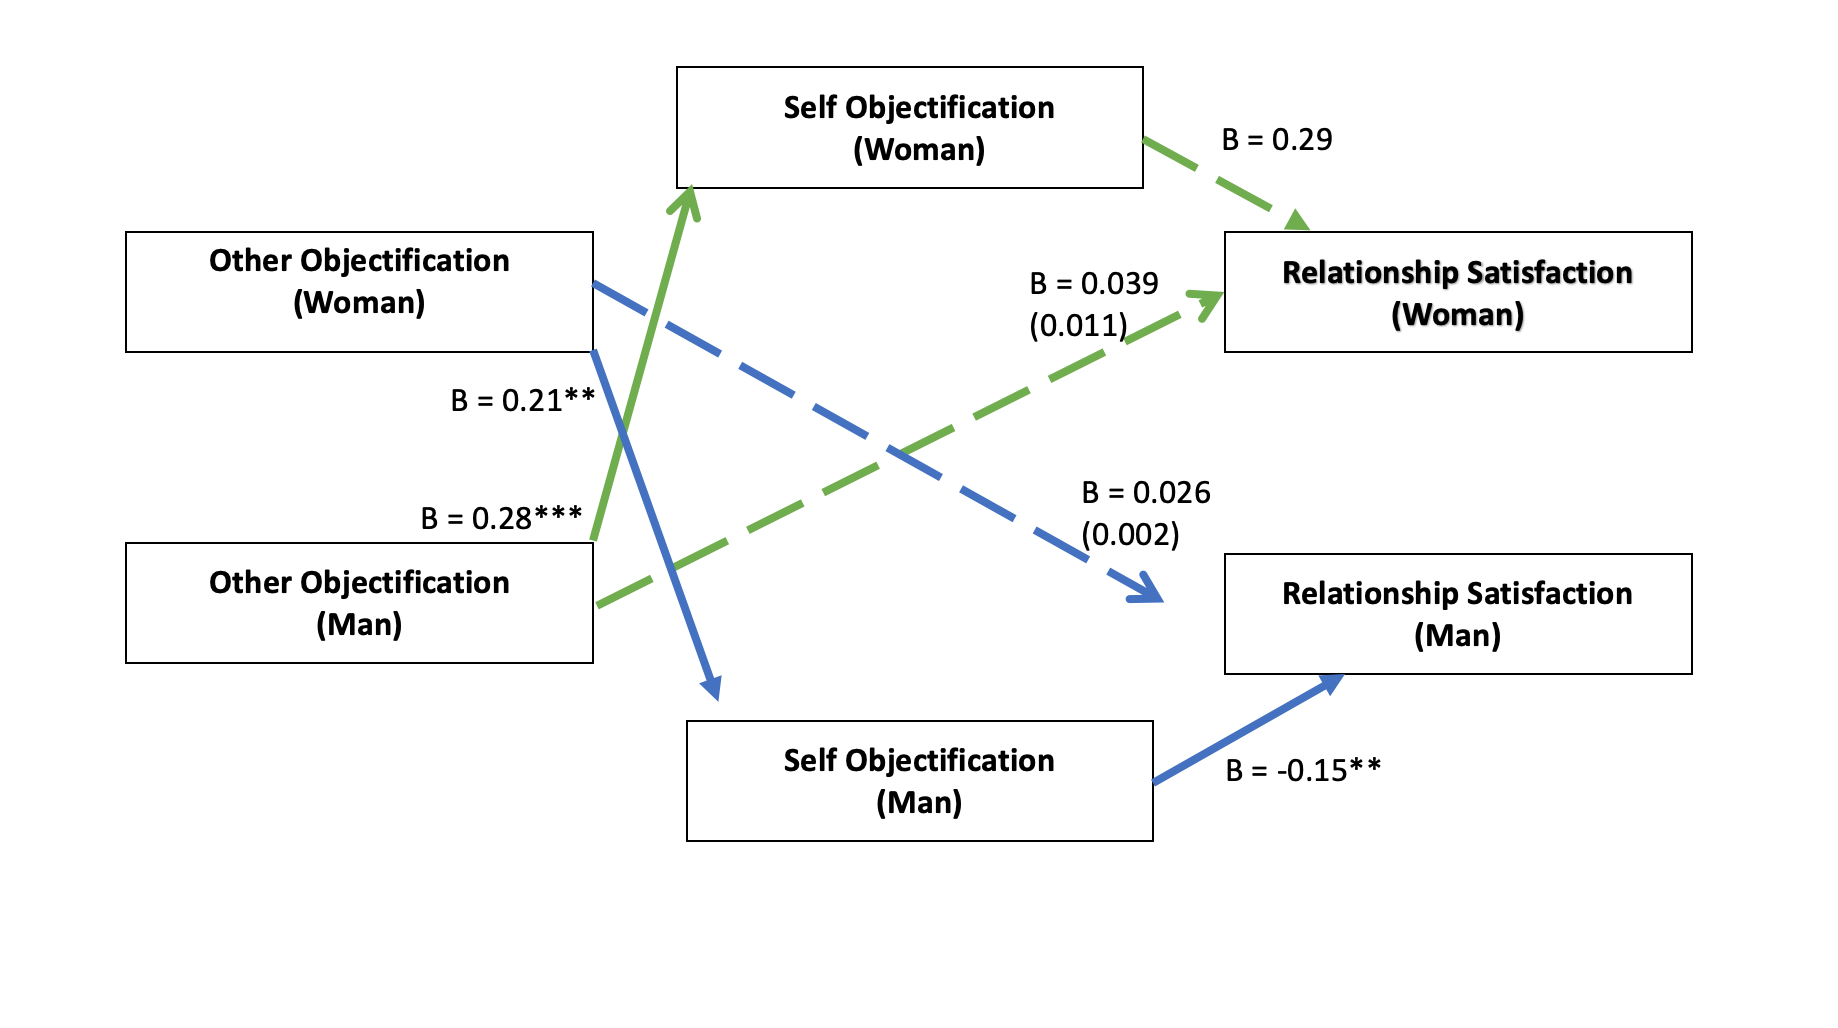
\includegraphics{Images/hypothesis_model_results.png}
\caption{Hypothesis}
\end{figure}

\begin{figure}
\centering
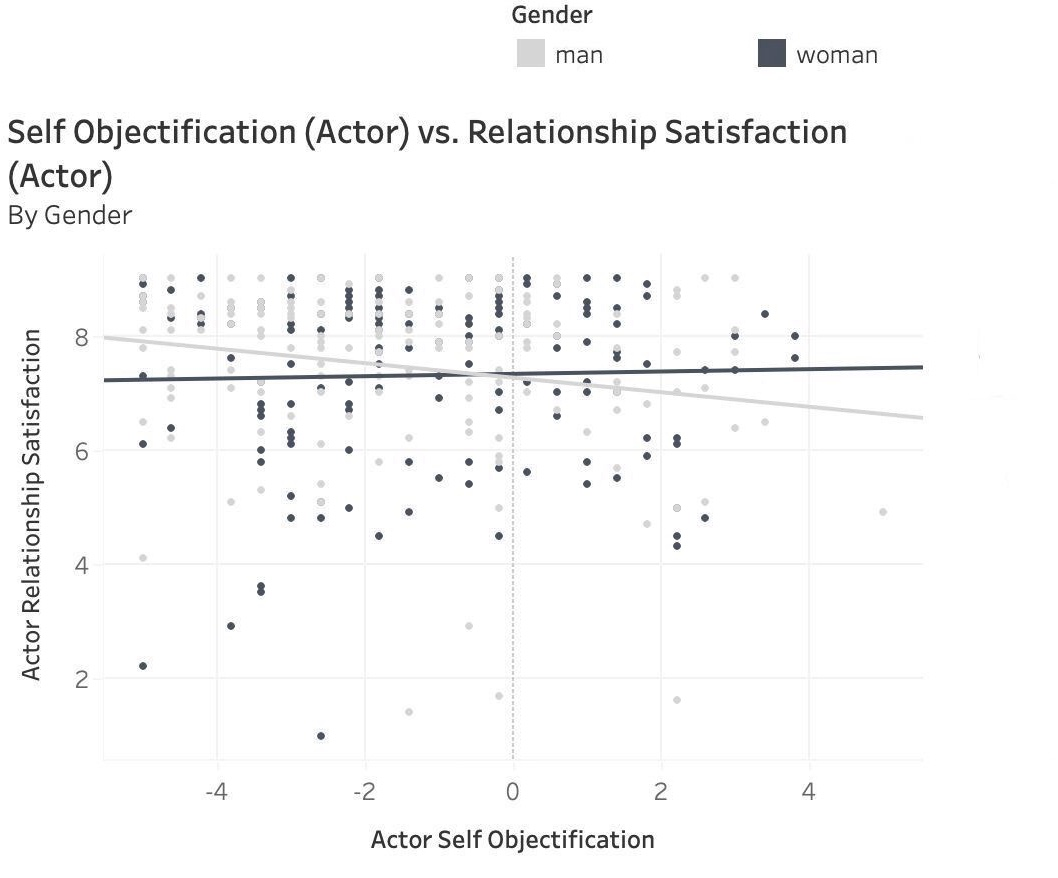
\includegraphics{Images/SO_RS_updated.png}
\caption{Self Objectification vs.~Relationship Satisfaction: Only the relationship between Self Objectification and Relationship Satisfaction was significant for males, that is, the more males in heterosexual relationships self objectify, the less satisfied they are with their relationships on average}
\end{figure}

\centering

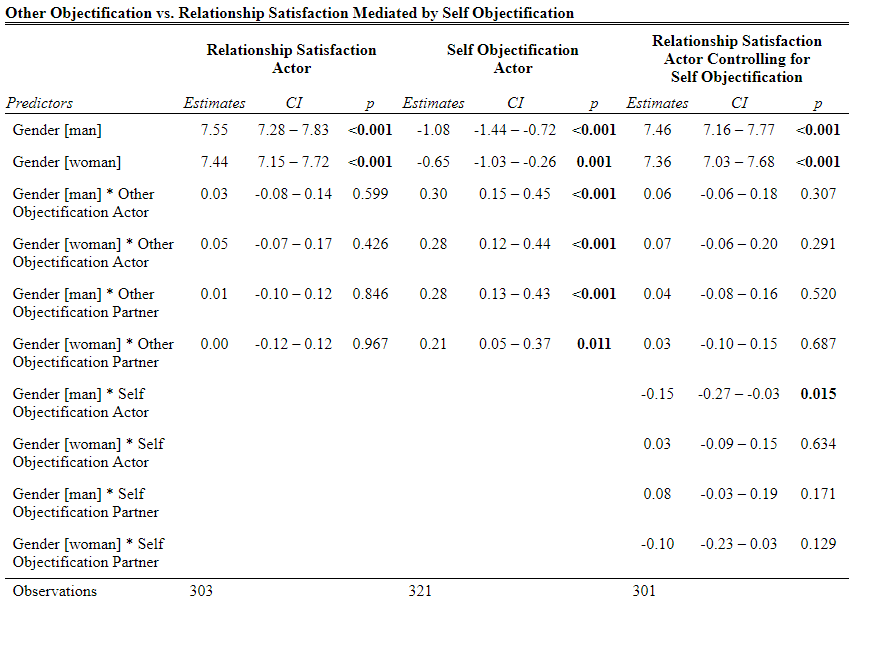
\includegraphics{Images/ResultsTableEdited.png} Table1

\begin{figure}
\centering
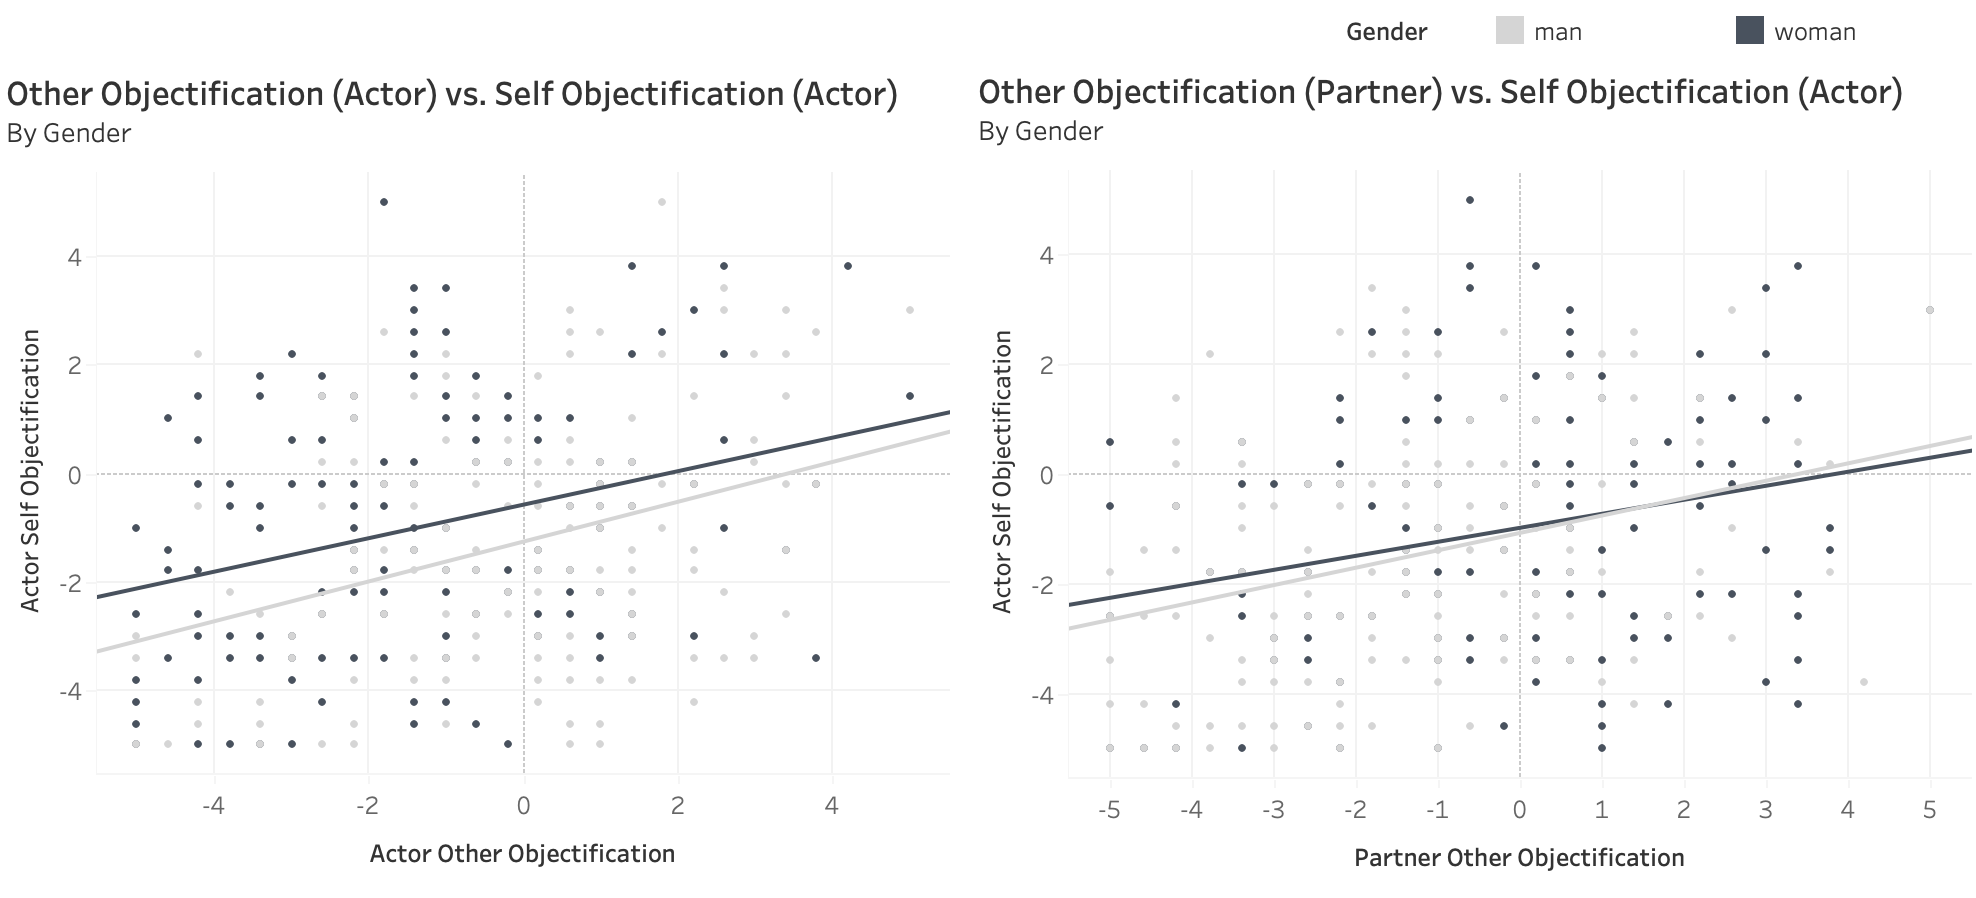
\includegraphics{Images/OO_vs_RSA.png}
\caption{Other Objectification vs.~Relationship Satisfaction}
\end{figure}

\hypertarget{discussion}{%
\section{Discussion}\label{discussion}}

Our results reported the effects of self-objectification and other objectification on a heterosexual couple's relationship satisfaction. Neither woman nor man's objectification of partner had a significant effect on woman or man's relationship satisfaction. This indicates that if a woman or man were to objectify their partner, their partner would not experience a significant increase or decrease to their relationship satisfaction because of the objectification.

We did not find any significance between a woman's objectification of herself and her own or her partner's relationship satisfaction. This means that a woman's objectification of herself does not influence her relationship satisfaction or the man's relationship satisfaction. We also found no association between men's self-objectification and women's relationship satisfaction but did find a significant negative effect for man's own relationship satisfaction. This tells us that a man's objectification of himself does not influence his partner's relationship satisfaction but does indeed hold a negative effect over his own, meaning that the more he objectifies himself, the less satisfied he will be with his relationship.

Each individual's objectification of a partner resulted in a significant positive effect on their partner's self-objectification, regardless of gender. This means that the more an individual objectifies their partner, the more their partner would tend to objectify themselves.

There is no evidence that supports an individual's objectification of a partner negatively influences the relationship satisfaction in both men and women in our study. These findings are unexpected since women are typically the ones who are more often being objectified by men (Sáez et al., 2019), especially since objectification has such a negative connotation in society (Terán et al., 2021). Our results are inconsistent with previous literature; in the current study, women's relationship satisfaction was unaffected by their own objectification, and being objectified by their partner.

Following that, it was even more surprising to find that men's relationship satisfaction was affected negatively by their own objectification of themselves, since men are usually portrayed to be less influenced by these relationship components (Gervais et al., 2011 ; Choma et al., 2010). A possible reason behind men being more affected by objectification in their relationship could be due to the fact that in day-to-day life, it is more common for men to be objectifying and for women to be objectified. Women have endured being objectified by multiple members of society, so when they experience objectification in their relationships, it is nothing new, and ceases to have an impact. However, when men are objectified by their partners, it is a new experience for them, and therefore are affected more deeply by it.

There is no evidence that supports self objectification meditates the association between partner objectification and relationship satisfaction in this study. Our results did find that an individual objectified by their partner is likely to objectify themselves, and an individual that objectifies their partner is likely to objectify themselves, both of which are consistent with previous literature (Strelan \& Hargreaves, 2005; Zurbriggen et al., 2011). Research shows there are associations between self objectification, partner objectification, and relationship satisfaction, so it was surprising that our findings suggest that self objectification does not mediate partner objectification and relationship satisfaction. It is possible that these hypotheses were not supported due to possible confounding variables, such as psychological intimacy as mentioned by Lameiras-Fernández et al. (2018).

Limitations for our study arrived in the initial phases of devising the methodology. We intended to evaluate how the effects of objectification varied across sexuality, more specifically, the differences between heterosexual (male-female) couples and same sex couples. However, due to the lack of same sex couples in our sample, we limited the scope of our study to only heterosexual couples, and evaluated how the effects varied across gender. Limiting our study to male-female dyads leaves a couple questions left to be answered, for example, ``Considering that Objectification Theory typically only discusses how women are affected by men's objectification of them, how do the effects of objectification change when no or only men are present in a relationship (same sex relationships)?''

The current research found that a man's objectification of himself hurts his own relationship satisfaction, and this was not found in women (contrary to objectification theory). Alternative explanations for this finding may be because men are often the perpetrators of objectification. Therefore, objectification may have a different influence on relationship satisfaction for men than for women. Due to the prioritization of women in objectification theory, we were limited in previous research regarding how a women's objectification of a man effects him. Additionally, women often prioritize other emotional support factors when determining their satisfaction with their relationship, alongside objectification. Our model did not include these emotional support factors that may help explain our results.

Future research studies could be conducted to address how the effects of objectification across gender may change when considering same sex couples. Moreover, since the current research highlights the effect objectification has on men, future research may consider conducting more studies that focus on men rather than women; the abundance of research of the objectification of women greatly overwhelms the research that may or may not suggest the same effects of objectification for men.

\hypertarget{conclusion}{%
\subsection{Conclusion}\label{conclusion}}

Overall, there were no differences between the association between partner objectification and relationship satisfaction between men and women. This is surprising, as it is not consistent with previous literature. In addition, there was no evidence that suggests that self objectification meditates the association between partner objectification and relationship satisfaction. An objectified partner's relationship satisfaction is not dependent on their relationship satisfaction. We hope for future studies to consider other variables that could mediate partner objectification and relationship satisfaction such as psychological intimacy, particularly in women due to insignificant findings in women's relationship satisfaction in this study. We did however find that a man's objectification of himself negatively impacts his own relationship satisfaction, and this was not found in women. Our study highlights men's perspectives of their own perceptions of themselves, while previous studies have highlighted women's self objectification in relation to their relationship satisfaction. We hope that in an effort to promote quality relationships, our research inspires greater consideration of self objectification in men, and in women.

\newpage

\hypertarget{references}{%
\section{References}\label{references}}

\begingroup
\setlength{\parindent}{-0.5in}
\setlength{\leftskip}{0.5in}

\hypertarget{refs}{}
\begin{CSLReferences}{1}{0}
\leavevmode\vadjust pre{\hypertarget{ref-braiker1979conflict}{}}%
Braiker, H. B., \& Kelley, H. H. (1979). Conflict in the development of close relationships. \emph{Social Exchange in Developing Relationships}, \emph{135}, 168.

\leavevmode\vadjust pre{\hypertarget{ref-choma2010self}{}}%
Choma, B. L., Visser, B. A., Pozzebon, J. A., Bogaert, A. F., Busseri, M. A., \& Sadava, S. W. (2010). Self-objectification, self-esteem, and gender: Testing a moderated mediation model. \emph{Sex Roles}, \emph{63}(9), 645--656.

\leavevmode\vadjust pre{\hypertarget{ref-cole2013body}{}}%
Cole, B. P., Davidson, M. M., \& Gervais, S. J. (2013). Body surveillance and body shame in college men: Are men who self-objectify less hopeful? \emph{Sex Roles}, \emph{69}(1), 29--41.

\leavevmode\vadjust pre{\hypertarget{ref-fredrickson1997objectification}{}}%
Fredrickson, B. L., \& Roberts, T.-A. (1997). Objectification theory: Toward understanding women's lived experiences and mental health risks. \emph{Psychology of Women Quarterly}, \emph{21}(2), 173--206.

\leavevmode\vadjust pre{\hypertarget{ref-gervais2011you}{}}%
Gervais, S. J., Vescio, T. K., \& Allen, J. (2011). When what you see is what you get: The consequences of the objectifying gaze for women and men. \emph{Psychology of Women Quarterly}, \emph{35}(1), 5--17.

\leavevmode\vadjust pre{\hypertarget{ref-lameiras2018objectifying}{}}%
Lameiras-Fernández, M., Fiske, S. T., Fernández, A. G., \& Lopez, J. F. (2018). Objectifying women's bodies is acceptable from an intimate perpetrator, at least for female sexists. \emph{Sex Roles}, \emph{79}(3), 190--205.

\leavevmode\vadjust pre{\hypertarget{ref-mahar2020partner}{}}%
Mahar, E. A., Webster, G. D., \& Markey, P. M. (2020). Partner--objectification in romantic relationships: A dyadic approach. \emph{Personal Relationships}, \emph{27}(1), 4--26.

\leavevmode\vadjust pre{\hypertarget{ref-meltzer2014tell}{}}%
Meltzer, A. L., \& McNulty, J. K. (2014). {``Tell me i'm sexy... And otherwise valuable''}: Body valuation and relationship satisfaction. \emph{Personal Relationships}, \emph{21}(1), 68--87.

\leavevmode\vadjust pre{\hypertarget{ref-meltzer2017women}{}}%
Meltzer, A. L., McNulty, J. K., \& Maner, J. K. (2017). Women like being valued for sex, as long as it is by a committed partner. \emph{Archives of Sexual Behavior}, \emph{46}(2), 475--488.

\leavevmode\vadjust pre{\hypertarget{ref-newheiser2010others}{}}%
Newheiser, A.-K., LaFrance, M., \& Dovidio, J. F. (2010). Others as objects: How women and men perceive the consequences of self-objectification. \emph{Sex Roles}, \emph{63}(9), 657--671.

\leavevmode\vadjust pre{\hypertarget{ref-noll1998mediational}{}}%
Noll, S. M., \& Fredrickson, B. L. (1998). A mediational model linking self-objectification, body shame, and disordered eating. \emph{Psychology of Women Quarterly}, \emph{22}(4), 623--636.

\leavevmode\vadjust pre{\hypertarget{ref-ramsey2015object}{}}%
Ramsey, L. R., \& Hoyt, T. (2015). The object of desire: How being objectified creates sexual pressure for women in heterosexual relationships. \emph{Psychology of Women Quarterly}, \emph{39}(2), 151--170.

\leavevmode\vadjust pre{\hypertarget{ref-ramsey2017sexualized}{}}%
Ramsey, L. R., Marotta, J. A., \& Hoyt, T. (2017). Sexualized, objectified, but not satisfied: Enjoying sexualization relates to lower relationship satisfaction through perceived partner-objectification. \emph{Journal of Social and Personal Relationships}, \emph{34}(2), 258--278.

\leavevmode\vadjust pre{\hypertarget{ref-saez2019objectification}{}}%
Sáez, G., Riemer, A. R., Brock, R. L., \& Gervais, S. J. (2019). Objectification in heterosexual romantic relationships: Examining relationship satisfaction of female objectification recipients and male objectifying perpetrators. \emph{Sex Roles}, \emph{81}(5), 370--384.

\leavevmode\vadjust pre{\hypertarget{ref-sciangula2009self}{}}%
Sciangula, A., \& Morry, M. M. (2009). Self-esteem and perceived regard: How i see myself affects my relationship satisfaction. \emph{The Journal of Social Psychology}, \emph{149}(2), 143--158.

\leavevmode\vadjust pre{\hypertarget{ref-strelan2005women}{}}%
Strelan, P., \& Hargreaves, D. (2005). Women who objectify other women: The vicious circle of objectification? \emph{Sex Roles}, \emph{52}(9), 707--712.

\leavevmode\vadjust pre{\hypertarget{ref-strelan2018birds}{}}%
Strelan, P., \& Pagoudis, S. (2018). Birds of a feather flock together: The interpersonal process of objectification within intimate heterosexual relationships. \emph{Sex Roles}, \emph{79}(1), 72--82.

\leavevmode\vadjust pre{\hypertarget{ref-teng2015sexual}{}}%
Teng, F., Chen, Z., Poon, K.-T., \& Zhang, D. (2015). Sexual objectification pushes women away: The role of decreased likability. \emph{European Journal of Social Psychology}, \emph{45}(1), 77--87.

\leavevmode\vadjust pre{\hypertarget{ref-teran2021relational}{}}%
Terán, L., Jiao, J., \& Aubrey, J. S. (2021). The relational burden of objectification: Exploring how past experiences of interpersonal sexual objectification are related to relationship competencies. \emph{Sex Roles}, \emph{84}(9), 610--625.

\leavevmode\vadjust pre{\hypertarget{ref-visser2014enjoyment}{}}%
Visser, B. A., Sultani, F., Choma, B. L., \& Pozzebon, J. A. (2014). Enjoyment of sexualization: Is it different for men? \emph{Journal of Applied Social Psychology}, \emph{44}(7), 495--504.

\leavevmode\vadjust pre{\hypertarget{ref-zurbriggen2011self}{}}%
Zurbriggen, E. L., Ramsey, L. R., \& Jaworski, B. K. (2011). Self-and partner-objectification in romantic relationships: Associations with media consumption and relationship satisfaction. \emph{Sex Roles}, \emph{64}(7), 449--462.

\end{CSLReferences}

\endgroup


\end{document}
